\chapter{Linebreeding}
\label{cha:Lush_Chapter_23}
\index{Inbreeding|(}
\index{Linebreeding|(}
\index{Relationship|(}

The word ``linebreeding'' is in common use among breeders of purebred
stock. It bears a good reputation and in that respect is in marked
contrast with ``in breeding.'' Linebreeding is mating animals so that
their descendants will be kept closely related to some animal regarded
as unusually desirable. It is accomplished by using for parents animals
which are both closely related to the admired ancestor but are little if at
all related to each other through any other ancestors. If both parents
are descended from the animal toward which the linebreeding is being
directed, they are related to each other and their mating is a form of
inbreeding in the broad sense of the word. If a man says an animal is
linebred, this instantly calls forth the question: ``Linebred to what?''
In fact, he will not often make such an incomplete statement as that an
animal ``is linebred.'' He will say that this bull is ``a linebred Domino''
or these ``are linebred Anxiety cattle'' or ``this bull is linebred to Prizemere
9th.'' The use of the term linebred almost carries with it the necessity
of specifying the animal or group of closely related animals toward
which the breeding is directed.

Linebreeding thus differs from other forms of inbreeding primarily
in that it is directed toward maintaining a high relationship to some
chosen ancestor and secondarily, in that it is usually less intense than
the most extreme inbreeding which might be practiced. Relationship
to the admired ancestor rather than intensity of inbreeding is dominating
the breeder's thought when he uses the term linebreeding, even
though this same breeder if he were asked for a formal definition of
linebreeding might give one which would mention nothing but the
intensity of the inbreeding.

The pedigrees below show the difference between linebreeding and
some other forms of inbreeding. The parents of \textit{X} are double first
cousins, having the same four grandparents. The parents of \textit{Y} are half
brother and sister. \textit{Z} is produced by mating a male to his own granddaughter.
\textit{W} is produced by mating a sire to his daughter out of one of
his own daughters. The intensity of the inbreeding is the same for \textit{X}, \textit{Y},
and \textit{Z}. Yet \textit{X} would rarely if ever be called linebred. Its sire and its dam
are related through four different ancestors which, so far as the pedigree
shows, may belong to four unrelated strains. If a breeder were to
call \textit{X} linebred, he would have to say that it was linebred to four different
lines at once, which is something of a contradiction in terms. He
would call \textit{Y} linebred to \textit{M} because \textit{K} and \textit{L} are related only through
\textit{M}, and \textit{Y} has been kept almost as closely related to \textit{M} as its parents
were. \textit{Z} is even more clearly a case of linebreeding because it is more
closely related to \textit{M} than \textit{Y} is, although no more intensely inbred. Many
breeders would call \textit{W} inbred in stead of linebred because the intensity
of its inbreeding is so high. Others would call it ``intensely linebred to
M,'' since all of its inbreeding is focused on M and it contains 87\nicefrac{1}{2}
percent of the blood of \textit{M} -- a relationship of 75 per cent after allowing for
\textit{W}'s inbreeding.\index{Inbreeding|)}\footnote{For other illustrations see Iowa Agr. Exp . Sta.,
Bul. 301, \textit{Linebreeding}.}

\begin{figure}
	\centering
    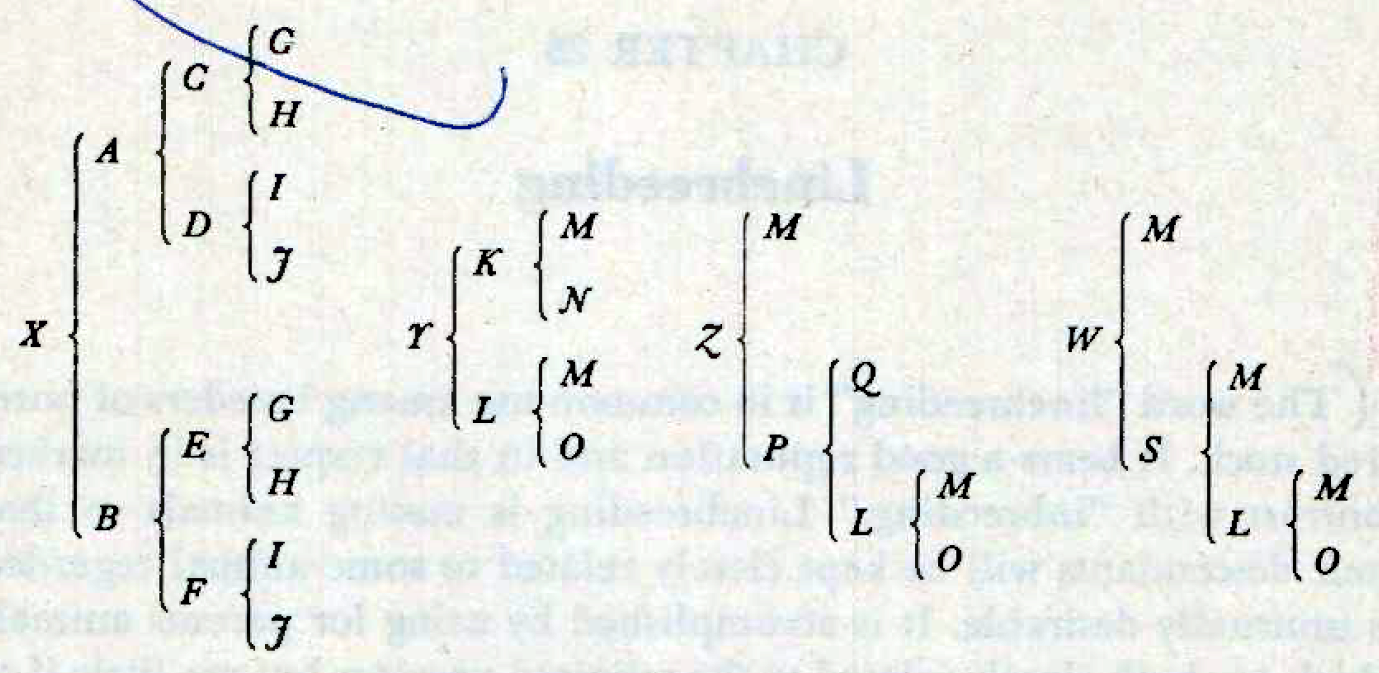
\includegraphics[width=\textwidth]{Page_300.png}
    \label{fig:Lush_Figure_Page_300}
\end{figure}

\section*{WHY LINEBREEDING IS PRACTICED}

Animals do not live long enough for the breeder to get all the sons
and daughters he wants from the best ones. Often an animal is old or
even dead before its real superiority is recognized . If its sons and
daughters are mated to unrelated individuals, the offspring will get
only about one -fourth of their inheritance from this outstanding grandparent.
If these in turn are mated to unrelated individuals, the influence
of the outstanding ancestor is again halved. Unless some form of
linebreeding is practiced, it is only a matter of three or four generations
until even the most outstanding animal's influence is so scattered and
diluted that no one descendant is very much like it. Linebreeding takes
advantage of the laws of probability as they affect Mendelian inheritance
to hold the expected amount of inheritance from an admired
ancestor at a nearly constant level instead of letting it be halved with
each generation, as would happen if all the matings were outbreeding.
Linebreeding provides, so to speak, a ratchet mechanism for holding
any gains already made by selection, while attempting to make further
gains.

Linebreeding also builds up homozygosity and prepotency within
the herd where it is practiced, just as other kinds of inbreeding do. It is
no more effective than other forms of inbreeding in this respect except
that, on account of the selection of the ancestors toward which the
inbreeding is directed, the \index{Homozygosis|}homozygosis produced by linebreeding is
more apt to be for desired traits than is the case with undirected
inbreeding. Linebreeding tends to separate the breed into distinct families,
each closely related to some admired ancestor, between which
effective selection can be practiced.

\section*{WHEN LINEBREEDING SHOULD BE PRACTICED}

The better the animals in a breeder's herd, the more reason he has
for linebreeding to them. The most vulnerable part in the linebreeding
program is whether the breeder is right when he decides which of the
animals recently used in his herd really were extraordinarily good ones.
If he can select the good from among the others with a high degree of
accuracy, linebreeding will be a powerful tool in his hands. If his judgment
about which animals were good is only fair, then linebreeding has
only a little advantage over other forms of inbreeding.

Those who can best afford to linebreed are breeders whose herds or
flocks are already distinctly superior to the general average of their
breed. If, by wise choice or lucky chance, such a breeder has used on
good dams a sire whose offspring turn out to be even better than their
dams, such a breeder ought to linebreed at once and strongly to this
sire while the animal is yet alive. If it is already dead when he discovers
how good it was, then he should hasten to linebreed to it while it still
has many sons and daughters by which such linebreeding can be accomplished.
While an animal is still living, the possibility of producing offspring
more closely related to it than any which yet exist remains open.
If a sire is thought good enough to make the risk worth taking, he can
be mated to his daughters and granddaughters generation after generation,
as seems to have been the intention of those who bred Blackcap
Empress (Figure~\ref{fig:Lush_Figure_30}). But after an animal dies the limit of relationship
to it which can be attained in future animals is only that of its closest
relatives then living. Even that is a limit only to be approached. If an
animal is dead by the time we realize how good it was and if there are
no living animals more closely related to it than 50 per cent, then there
is no possible way to produce animals more closely related to it than
that. If we have let its sons and daughters and full brothers and sisters
die before we wake up to its merit and there are left no living animals
more closely related to it than 25 per cent, then we cannot produce any
future animals more closely related to it than that -- hence the importance
of starting the linebreeding while there is time to do so effectively.
Figure~\ref{fig:Lush_Figure_39} shows a case where that seems to have been
planned definitely.

\begin{figure}
	\centering
    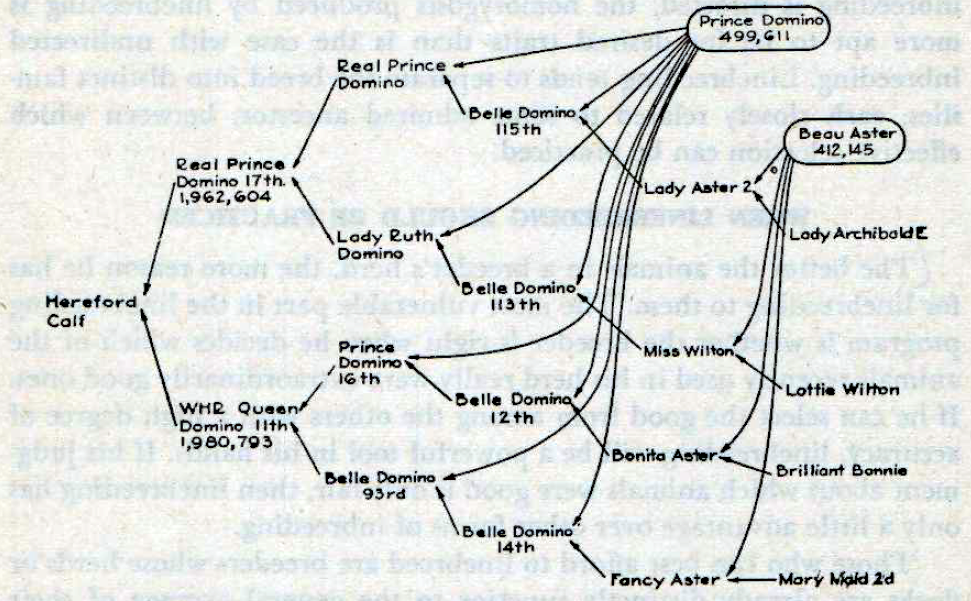
\includegraphics[width=\textwidth]{Figure_39.png}
    \caption{Long-continued and deliberate linebreeding to Prince Domino with a
			 very little linebreeding also to Beau Aster. Pedigrees like this do
			 not ``just happen.'' It took planning to get four different
			 grandparents with so nearly identical pedigrees and to bring them
			 together in this way without any secondary linebreeding.}
    \label{fig:Lush_Figure_39}
\end{figure}

\nowidow
It is an open question whether breeders with purebred herds of average
merit can afford to do much linebreeding. Certainly there are many
good animals in such herds and much good inheritance which stands
small chance of being kept together unless linebreeding is practiced. On
the other hand, if the initial merit of the herd was only average, one
must count on a certain amount of inbreeding degeneration which
might bring the average merit of the herd below the level of the breed.
The question at issue is whether the increased effectiveness of selection
possible under linebreeding will be more than enough to offset the
expected amount of inbreeding degeneration.

\index{Inbreeding!dangers of|(}
\index{Relationship|)}
Breeders of grades cannot often afford to linebreed. The inbreeding
risk involved is probably just a little greater for them than for the
breeder of purebreds on account of the slightly greater heterozygosis of
the grades. Even if a breeder of grades is successful at linebreeding, he
cannot sell at a premium the increased prepotency and uniformity
which would thus be put into his animals. He does not have the chance
to gain as much by successful linebreeding as breeders of purebreds do.
However, it sometimes happens that the breeder of grades uses a sire
whose offspring turn out to be so much better th:i.n their dams that the
inbreeding risk of using the sire on his own granddaughters or even on
his own daughters seems worth taking. It seems likely that there are
more breeders of grades who lose by failing to conserve a good sire than
there are who lose by getting too many of the usual bad results of
inbreeding while trying to linebreed to a good sire. For the breeders of
grades, the certain merit of the animal to which he might linebreed
needs to be further above the probable merit of the next sire which he
would otherwise use than is the case with the breeder of purebreds.

\index{Epistatic effects}
Linebreeding is especially needed where there is much epistasis.
Wherever a desired characteristic depends on a combination of genes
which individually have undesired effects, those gene combinations
tend to be scattered at each segregation. If inbreeding has made the
family homozygous for several of these genes, the whole combination
has more chance of being transmitted to enough of the offspring to
permit its becoming established in that family. If the form of inbreeding
used is linebreeding, with selection constantly directed toward keeping
the family closely related to animals which once showed that
desirable combination, the chances of recovering the whole combination
among the descendants are much better than if the descendants
were continually outbred to unrelated animals. Outbreeding would
increase the likelihood that this particular combination of genes would
be scattered into its constituent and individually useless parts. Linebreeding
is the only very promising way of securing desirable gene
combinations differing from the most frequent type of the breed by
much more than four or five gene substitutions, each of which is harmful
if made one at a time but beneficial if all can be made at once. That
is, linebreeding is the answer to the situation pictured in
Figures~\ref{fig:Lush_Figure_20} and \ref{fig:Lush_Figure_21}, in chapter
12, where it was pointed out that selection could carry a
population to the nearest peak of desirability but could not carry it to a
peak of higher desirability across an intervening valley which was more
than a few gene substitutions in width.
\index{Inbreeding!dangers of|)}

\section*{DANGERS OF LINEBREEDING}

The breeder may have the wrong ideal and be breeding toward a
type which has a lower sale value than some other type. Of course this
same danger exists in all other breeding systems. But, since linebreeding
is more effective in carrying the breeder toward his goal, it is more
important for a breeder practicing linebreeding to be sure of his goal
than for one who is breeding by individuality alone.

Linebreeding may be so intense that genes will become homozygous
more rapidly than the breeder can discard the undesired homozygotes.
The inbreeding may thus result in fixing in his herd some undesired
genes in spite of all the selecting he can do against them. Whether this
will happen depends not only on the inbreeding intensity but on the
merit of the stock with which he starts and on the skill which he exercises
in his selection, including such use as he makes of progeny tests,
pedigree estimates, etc. Then, too, a part of the success or failure will
be due to the chance inherent in Mendelian inheritance whereby one
individual from a particular mating may happen to be a better or worse
individual than would ever be produced again from that same mating.

There is no magic about the linebreeding process which will automatically
produce good results. If selection is not practiced, a breeder
will generally do better to avoid linebreeding altogether, since he would
thereby avoid the inbreeding effect. But a breeder starting with good
stock and directing the linebreeding toward the best of the recent ancestors
in his herd can effect more improvement by selection while holding
the improvement he already has than would be possible if he were continually
outbreeding.

\begin{figure}
	\centering
    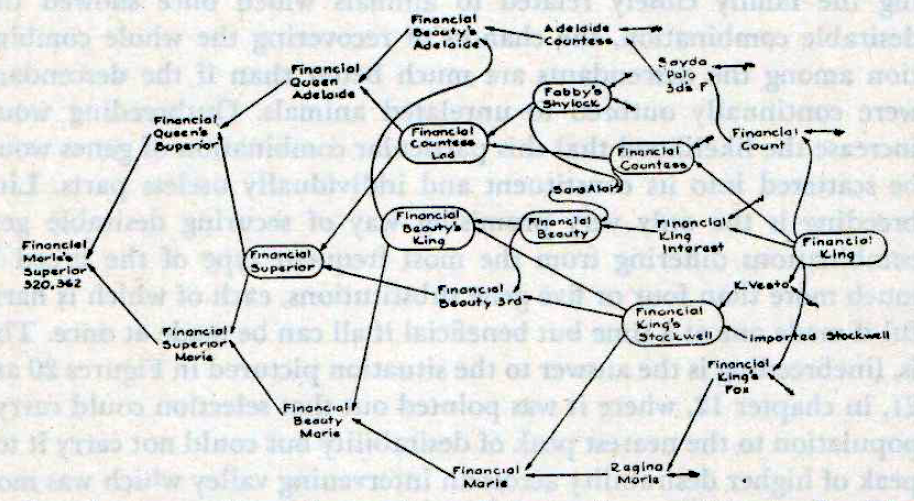
\includegraphics[width=\textwidth]{Figure_40.png}
    \caption{Long-continued linebreeding within the Financial King family of Jerseys.
			 Much of the linebreeding here is secondary and to recent animals such as
			 Financial Superior, Financial Countess Lad, and Financial Beauty's King.}
    \label{fig:Lush_Figure_40}
\end{figure}

If one wishes to linebreed purely to one animal, he must see to it
early that a large number of sons and daughters of that animal are
saved. Otherwise the time quickly comes when furth er linebreeding to
that ancestor also involves considerable linebreeding to some of its
descendants. Figures~\ref{fig:Lush_Figure_38}, \ref{fig:Lush_Figure_40},
and \ref{fig:Lush_Figure_41} show cases of that. There is no particular
lar reason why this secondary linebreeding should be avoided if the
animal toward which it is directed is an unusually good one. But, if the
herd is small and only one man is linebreeding to this line, there will be
only a few individuals in each generation. In some generations it will
happen that no one of those will be outstanding enough to justify linebreeding
to it. If the number of animals in this linebred strain or family
is very small, the breeder must either linebreed to some of those which
were not good enough to justify it, or else he will have to give up his
linebreeding plan and m.ake a distinct outcross. This is the intrinsic
danger of a permanent line breeding policy based on too small a herd. If
the herd is large enough, such secondary linebreeding can be avoided or
at least can be kept so small in amount in those generations when there
is no outstanding individual that it will be practically harmless. Hence,
a linebreeding plan which is to last more than two or three generations
without much risk requires the equivalent of a herd large enough to
justify keeping about three to five sires in use at all times.\footnote{These
figures are based on the $1/8M$ formula for loss of hetcrozygosis within
a closed group. (See Chap. 21.)} This might be one large herd; or several
breeders with small herds might co-operate in breeding toward the same line,
exchanging breeding stock with each other but rarely if ever introducing a
breeding animal from herds not in the group.

\begin{figure}
	\centering
    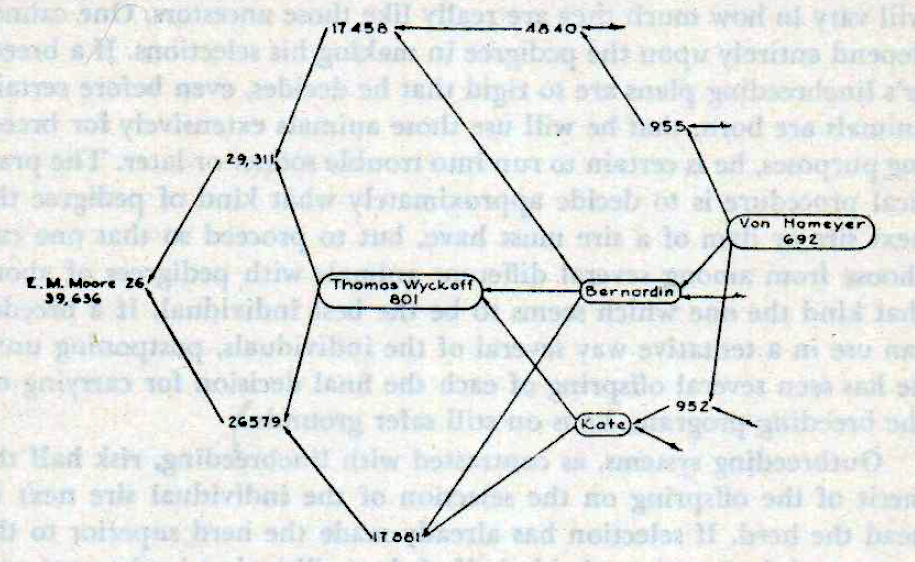
\includegraphics[width=\textwidth]{Figure_41.png}
    \caption{A Rambouillct pedigree in which one male is the center of the line breeding
			 in each generation.}
    \label{fig:Lush_Figure_41}
\end{figure}

\section*{GENETIC ASPECTS OF LINEBREEDING}
\index{Inbreeding|(}

Linebreeding, more than any other breeding system, combines selection
with inbreeding. In a certain sense, linebreeding is selection among
the ancestors rather than among living animals. Since many of the
ancestors being considered will have had several different offspring,
they arc to some extent proved sires and proved dams. The linebreeding
is, therefore, selecting from among progeny-tested\index{Progeny test} ancestors those
whose influence is to be preserved. This advantage is partly offset by the
fact that the individuals used to preserve the traits of their ancestors
will vary in how much they are really like those ancestors. One cannot
depend entirely upon the pedigree in making his selections. If a breeder's
linebreeding plans are so rigid that he decides, even before certain
animals are born, that he will use those animals extensively for breeding
purposes, he is certain to run into trouble sooner or later. The practical
procedure is to decide approximately what kind of pedigree the
next sire or dam of a sire must have, but to proceed so that one can
choose from among several different animals with pedigrees of about
that kind the one which seems to be the best individual. If a breeder
can use in a tentative way several of the individuals, postponing until
he has seen several offspring of each the final decision for carrying on
the breeding program, he is on still safer grounds.

\index{Outbreeding}
Outbreeding systems, as contrasted with linebreeding. risk half the
merit of the offspring on the selection of the individual sire next to
head the herd. If selection has already made the herd superior to the
average of the breed, probably half of that will be lost in the next generation
unless selection is again as effective as it was before. Every
breeder will occasionally make mistakes in his selections. The breeder
who continually practices outbreeding can therefore expect to have the
merit of his herd at times go far back toward the average of the breed.
One who wants to make and keep his herd far different from the average
of the breed to which it belongs must put some kind of a pedigree
barrier between it and the rest of the breed, so that the differences continually
being produced as successive sires are used will tend to accumulate
and not be halved with each successive sire. An analogy may make
that point clear. Water tends to seek its level. If there were no barriers
in the way, the level of the water in all the lakes of the world would
quickly seek the level of the ocean, just as the water in the rivers is
continually doing. The breeder who practices outbreeding is placing
no barriers, except his own skill at selecting, in the way of his herd's
tending toward the average level of the breed. The breeder who practices
linebreeding is to a considerable extent isolating his herd from
the rest of the breed, and its merit tends toward that of the isolated
group rather than toward that of the breed as a whole, just as the level
of the water in Lake Erie remains nearly constant but several hundred
feet above the level of the water in the ocean, even though water is
steadily flowing into it and out of it again.

\section*{SUMMARY}

Linebreeding is a form of inbreeding directed toward keeping the
offspring closely related to a highly admired ancestor. All inbreeding
not necessary for holding this relationship high is avoided as far as possible.
Hence, the intensity of the inbreeding is usually moderate in
linebreeding systems. Relationship to a chosen ancestor is the main
feature which distinguishes linebreeding from other forms of
inbreeding.

It is practiced to conserve the good traits of an outstanding sire or
dam among its descendants, increasing those descendants in numbers
without lessening their resemblance to this ancestor.

The more superior a breeder's herd or flock is to the average merit
of its breed the more reason he has to practice linebreeding to his very
best animals or to the very best of their recent ancestors.

The risk involved in linebreeding depends upon how much undesirable
inheritance is in the herd when the lincbreeding begins, upon
how skillful the breeder can be in his selections, how much use he can
make of progeny tests before he has to decide whether to use a sire
extensively, how large his herd is, and whether he must work alone . If
he can co-operate with several other breeders who are linebreeding to
closely related animals, he can get an occasional mild outcross from
them without disturbing his whole program.

Linebreeding is choosing which ancestors shall have their influence
conserved and spread through the whole herd and which ancestors shall
be allowed to diminish in importance with each generation until they
no longer have much effect.
\index{Inbreeding|)}
\index{Linebreeding|)}